\documentclass[a4paper,11pt]{article}
\usepackage{graphicx,url}
\usepackage[T1]{fontenc}
\usepackage[utf8]{inputenc}
\usepackage[brazil]{babel}
\usepackage{a4wide}
\usepackage{booktabs}
\graphicspath{{./imagens/}}
\title{\vspace{-4cm}Relatório 08 - Laboratório de Arquitetura de Computadores}
\author{Luiz Junio Veloso Dos Santos - Matricula: 624037}

\begin{document} 

\maketitle

\begin{enumerate}
    \item{O que é um arquivo fonte?}
        \begin{enumerate}
            \item{Um arquivo de texto que contém instruções de linguagem de programação.}
            \item{Um subdiretório que contém os programas.}
            \item{Um arquivo que contém dados para um programa.}
            \item{Um documento que contém os requisitos para um projeto.}
        \end{enumerate}
        \textbf{R: a) Um arquivo de texto\dots}

    \item{O que é um registro?}
        \begin{enumerate}
            \item{parte do sistema de computador que mantém o controle dos parâmetros do sistema.}
            \item{uma parte do processador que possui um padrão de bits.}
            \item{parte do processador que contém o seu número de série único.}
            \item{parte do bus de sistema que contém dados.}
        \end{enumerate}
        \textbf{R: a) parte do sistema de computador\dots}

    \item{Qual carácter que, na linguagem assembly do SPIM, inicia um comentário?}
        \begin{enumerate}
            \item{\#}
            \item{\%}
            \item{//}
            \item{*}
        \end{enumerate}
        \textbf{R: a) \#}

    \item{Quantos bits há em cada instrução de máquina MIPS?}
        \begin{enumerate}
            \item{8}
            \item{16}
            \item{32}
            \item{instruções diferentes possuem diferentes comprimentos.}
        \end{enumerate}
        \textbf{R: c) 32}

    \item{Quando você abre um arquivo de origem a partir do menu Arquivo SPIM, quais as duas coisas que 
            acontecem? }
        \begin{enumerate}
            \item{O arquivo está carregado na memória e começa a execução.}
            \item{SPIM é iniciado e o arquivo é aberto no editor.}
            \item{O arquivo é montado em instruções de máquina, e as instruções de maquina são
                    carregados na memória do SPIM.}
            \item{O programa é executado e os resultados são salvos em disco.}
        \end{enumerate}
        \textbf{R: c) O arquivo é montado\dots }

    \item{O que é o contador de programa?}
        \begin{enumerate}
            \item{um registrador que mantém a conta do número de erros durante a execução de um
                    programa}
            \item{uma parte do processador que contém o endereço da primeira palavra de dados.}
            \item{uma variável na montadora que os números das linhas do arquivo de origem.}
            \item{parte do processador que contém o endereço da próxima instrução de maquina para ser
                    obtida.}
        \end{enumerate}
        \textbf{R: d) parte do processador que contém o endereço da proxima instrução\dots}

    \item{Ao pressionar a tecla F10 para executar uma instrução, quanto será adicionado ao contador de
            programa?}
        \begin{enumerate}
            \item{1}
            \item{2}
            \item{4}
            \item{8}
        \end{enumerate}
        \textbf{R: c) 4}

    \item{O que é uma diretiva, tal como a diretiva .text?}
        \begin{enumerate}
            \item{Uma instrução em linguagem assembly que resulta em uma instrução em linguagem de
                    máquina.}
            \item{uma das opções de menu do sistema SPIM.}
            \item{uma instrução em linguagem de maquina que faz com que uma operação sobre os dados ocorra.}
            \item{uma declaração que diz o montador algo sobre o que o programador quer, mas não
                    corresponde diretamente a uma instrução de máquina.}
        \end{enumerate}
        \textbf{R: d) uma declaração que diz o montador algo sobre\dots}

    \item{O que é um endereço simbólico?}
        \begin{enumerate}
            \item{um local de memória que contém dados simbólicos.}
            \item{um byte na memória que contém o endereço de dados.}
            \item{símbolo dado como argumento para uma directiva.}
            \item{um nome usado no código fonte em linguagem assembly para um local na memória.}
        \end{enumerate}
        \textbf{R: c) um simbólo dado como argumento para uma directiva.}

        \newpage 

    \item{Em qual endereço o simulador SPIM coloca a primeira instrução de máquina quando ele está sendo
            executado com a opção Bare Machine ligada?}
        \begin{enumerate}
            \item{0x00000000}
            \item{0x00400000}
            \item{0x10000000}
            \item{0xFFFFFFFF}
        \end{enumerate}
        \textbf{R: b) 0x00400000}

    \item{Algumas instruções de máquina possuem uma constante como um dos operandos. Como é chamado tal
            operando?}
        \begin{enumerate}
            \item{operando imediato}
            \item{operando embutido}
            \item{operando binário}
            \item{operando de máquina}
        \end{enumerate}
        \textbf{R: a) operando imediato}

    \item{Como é chamada uma operação lógica executada entre bits de cada coluna dos operandos para
            produzir um bit de resultado para cada coluna?}
        \begin{enumerate}
            \item{operação lógica}
            \item{operação bitwise}
            \item{operação binária}
            \item{operação coluna}
        \end{enumerate}
        \textbf{R: b) operação bitwise}

    \item{Quando uma operação é de fato executada, como estão os operandos na ALU?}
        \begin{enumerate}
            \item{Pelo menos um operando deve ser de 32 bit.}
            \item{Cada operando pode ser de qualquer tamanho.}
            \item{Ambos operandos devem vir de registros.}
            \item{Cada um dos registradores deve possuir 32 bit.}
        \end{enumerate}
        \textbf{R: d) Cada um dos registradores\dots}

    \item{Dezesseis bits de dados de uma instrução de `ori' são usados como um operando imediato. Durante
            execução, o que deve ser feito primeiro?}
        \begin{enumerate}
            \item{Os dados são estendidos em zero à direita por 16 bits.}
            \item{Os dados são estendidos em zero à esquerda por 16 bits.}
            \item{Nada precisa ser feito.}
            \item{Apenas 16 bits são usados pelo outro operando.}
        \end{enumerate}
        \textbf{R: b) Os dados são estendidos em zero à esquerda\dots}

    \item{Qual o nome para um padrão de bits copiados em um registrador?}
        \begin{enumerate}
            \item{load.}
            \item{filled.}
            \item{stuffed.}
            \item{fixed.}
        \end{enumerate}
        \textbf{R: a) load}

    \item{Qual das instruções seguintes armazenam no registrador \$5 um padrão de bits que
            representa positivo 48?}
        \begin{enumerate}
            \item{ori \$5, \$0, 0x48}
            \item{ori \$5, \$5, 0x48}
            \item{ori \$5, \$0, 48}
            \item{ori \$0, \$5, 0x48}
        \end{enumerate}
        \textbf{R: c) ori \$5, \$0, 48}

    \item{A instrução de `ori' pode armazenar o complemento de dois de um número em um registrador?}
        \begin{enumerate}
            \item{Não.}
            \item{Sim.}
        \end{enumerate}
        \textbf{R: b) Sim}

    \item{Qual das instruções seguintes limpa todos os bits no registrador \$8 com exceção do byte de
            baixa ordem que fica inalterado?}
        \begin{enumerate}
            \item{ori \$8, \$8, 0xFF}
            \item{ori \$8, \$0, 0x00FF}
            \item{xori \$8, \$8, 0xFF}
            \item{andi \$8, \$8, 0xFF}
        \end{enumerate}
        \textbf{R: d) andi \$8, \$8, 0xFF }

    \item{Qual é o resultado de um `ou exclusivo' de padrão sobre ele mesmo?}
        \begin{enumerate}
            \item{Todos os bits em zero.}
            \item{Todos os bits em um.}
            \item{O padrão original utilizado.}
            \item{O resultado é o contrário do original.}
        \end{enumerate}
        \textbf{R: a) Todos os bits em zero.}
        \newpage
    \item{Todas as instruções de máquina têm os mesmos campos?}
        \begin{enumerate}
            \item{Não. Diferentes de instruções de máquina possuem campos diferentes.}
            \item{Não. Cada instrução de máquina é completamente diferente de qualquer outra.}
            \item{Sim. Todas as instruções de máquina têm os mesmos campos na mesma ordem.}
            \item{Sim. Todas as instruções de máquina têm os mesmos campos, mas eles podem estar em ordens
                    diferentes.}
        \end{enumerate}
        \textbf{R: a) Não.\dots}
\end{enumerate}

\newpage

\begin{figure}[!ht]
    \caption{Programa 1}
    \centering
    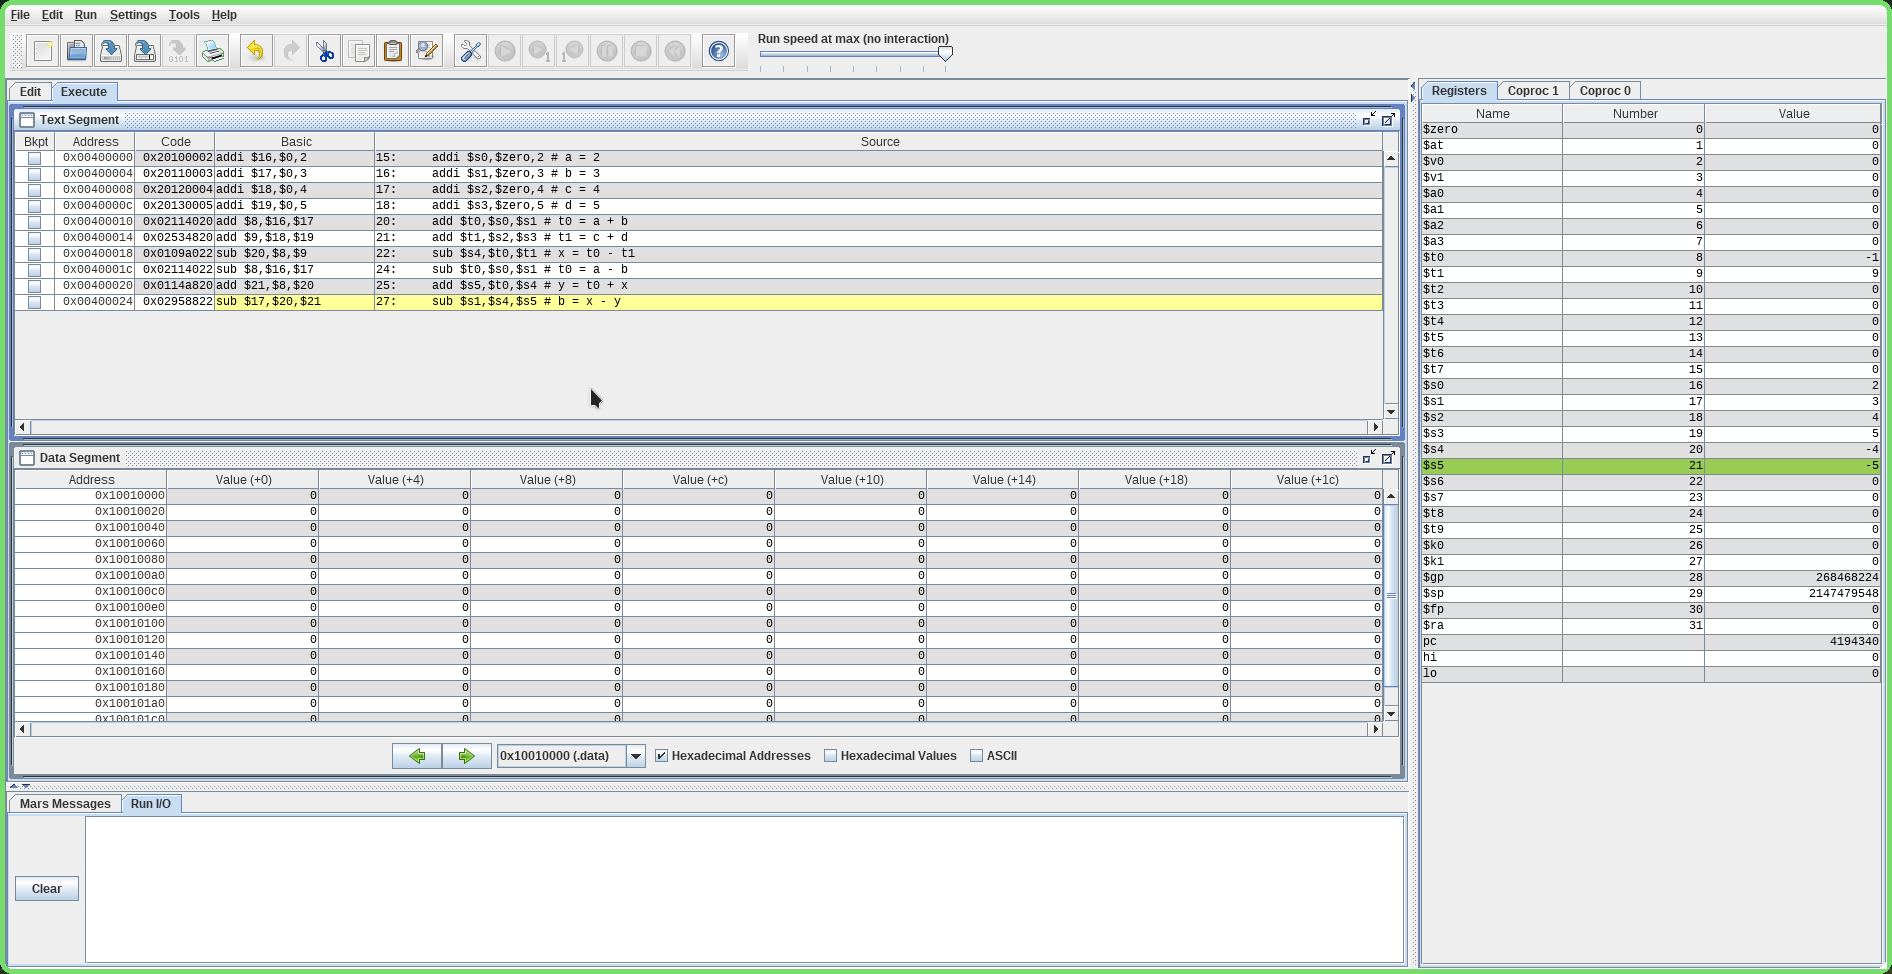
\includegraphics[width=1\textwidth]{programa1}
\end{figure}
\begin{figure}[!ht]
    \caption{Programa 2}
    \centering
    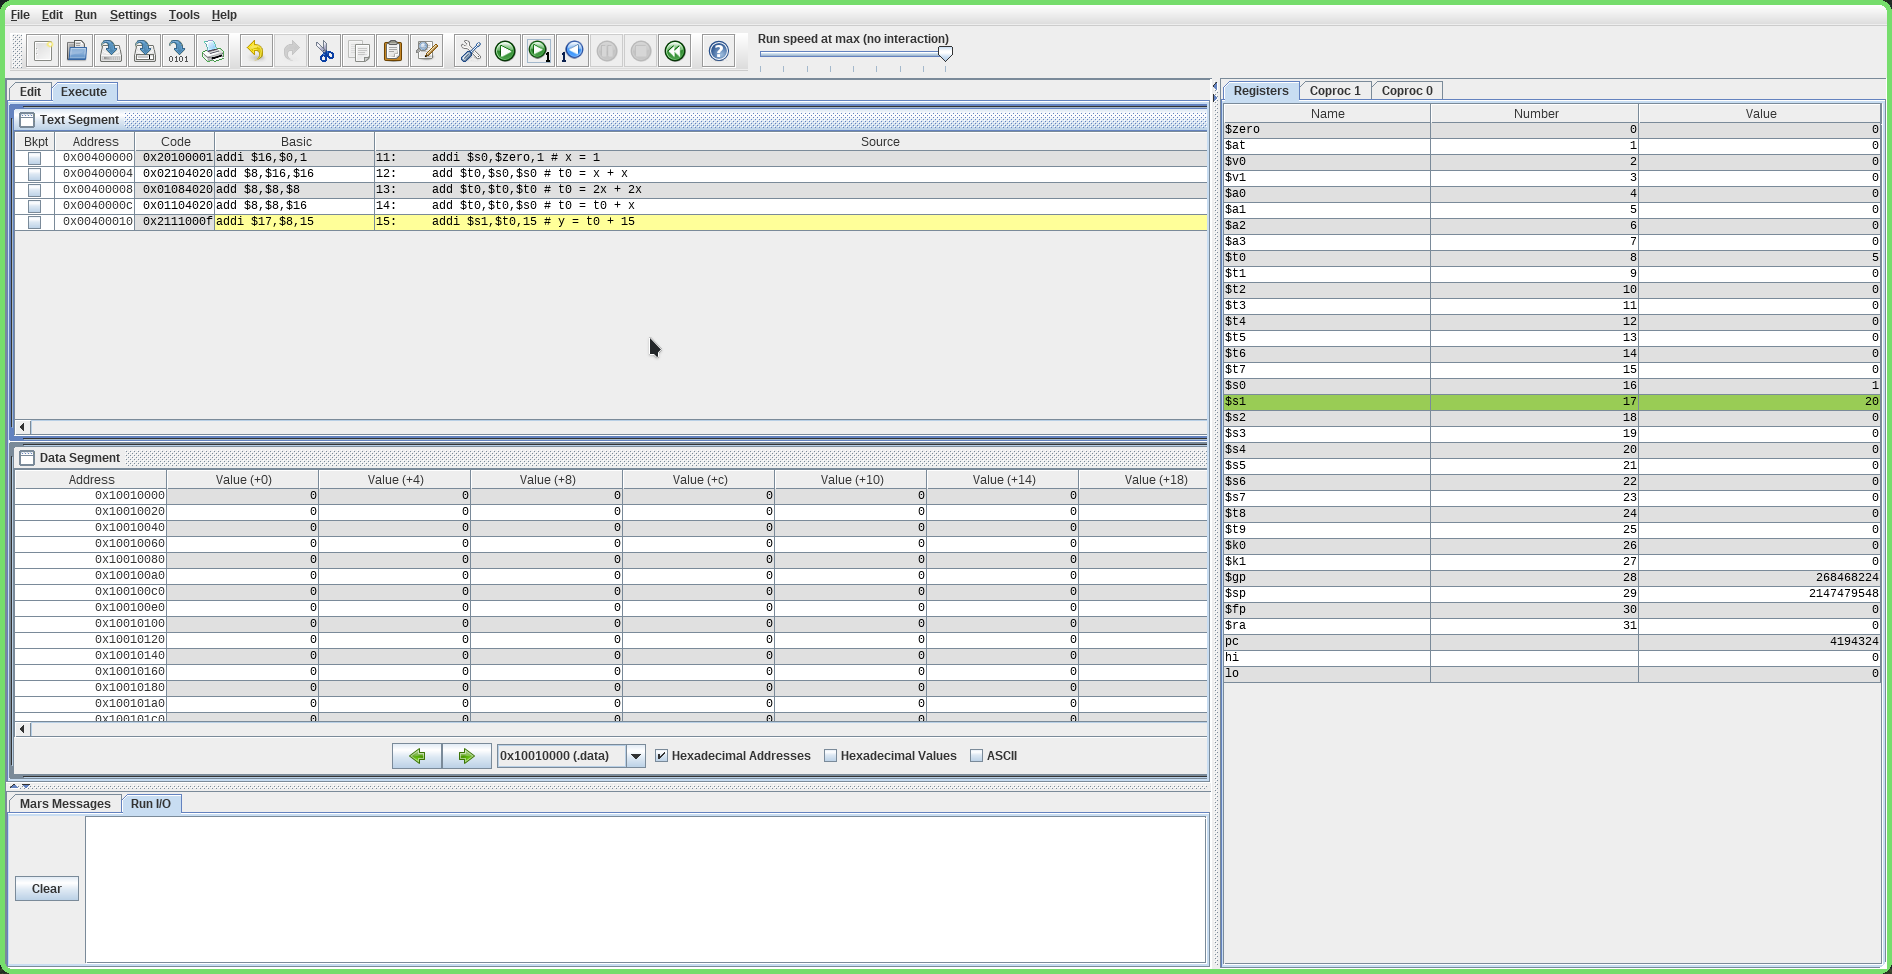
\includegraphics[width=1\textwidth]{programa2}
\end{figure}
\begin{figure}[!ht]
    \caption{Programa 3}
    \centering
    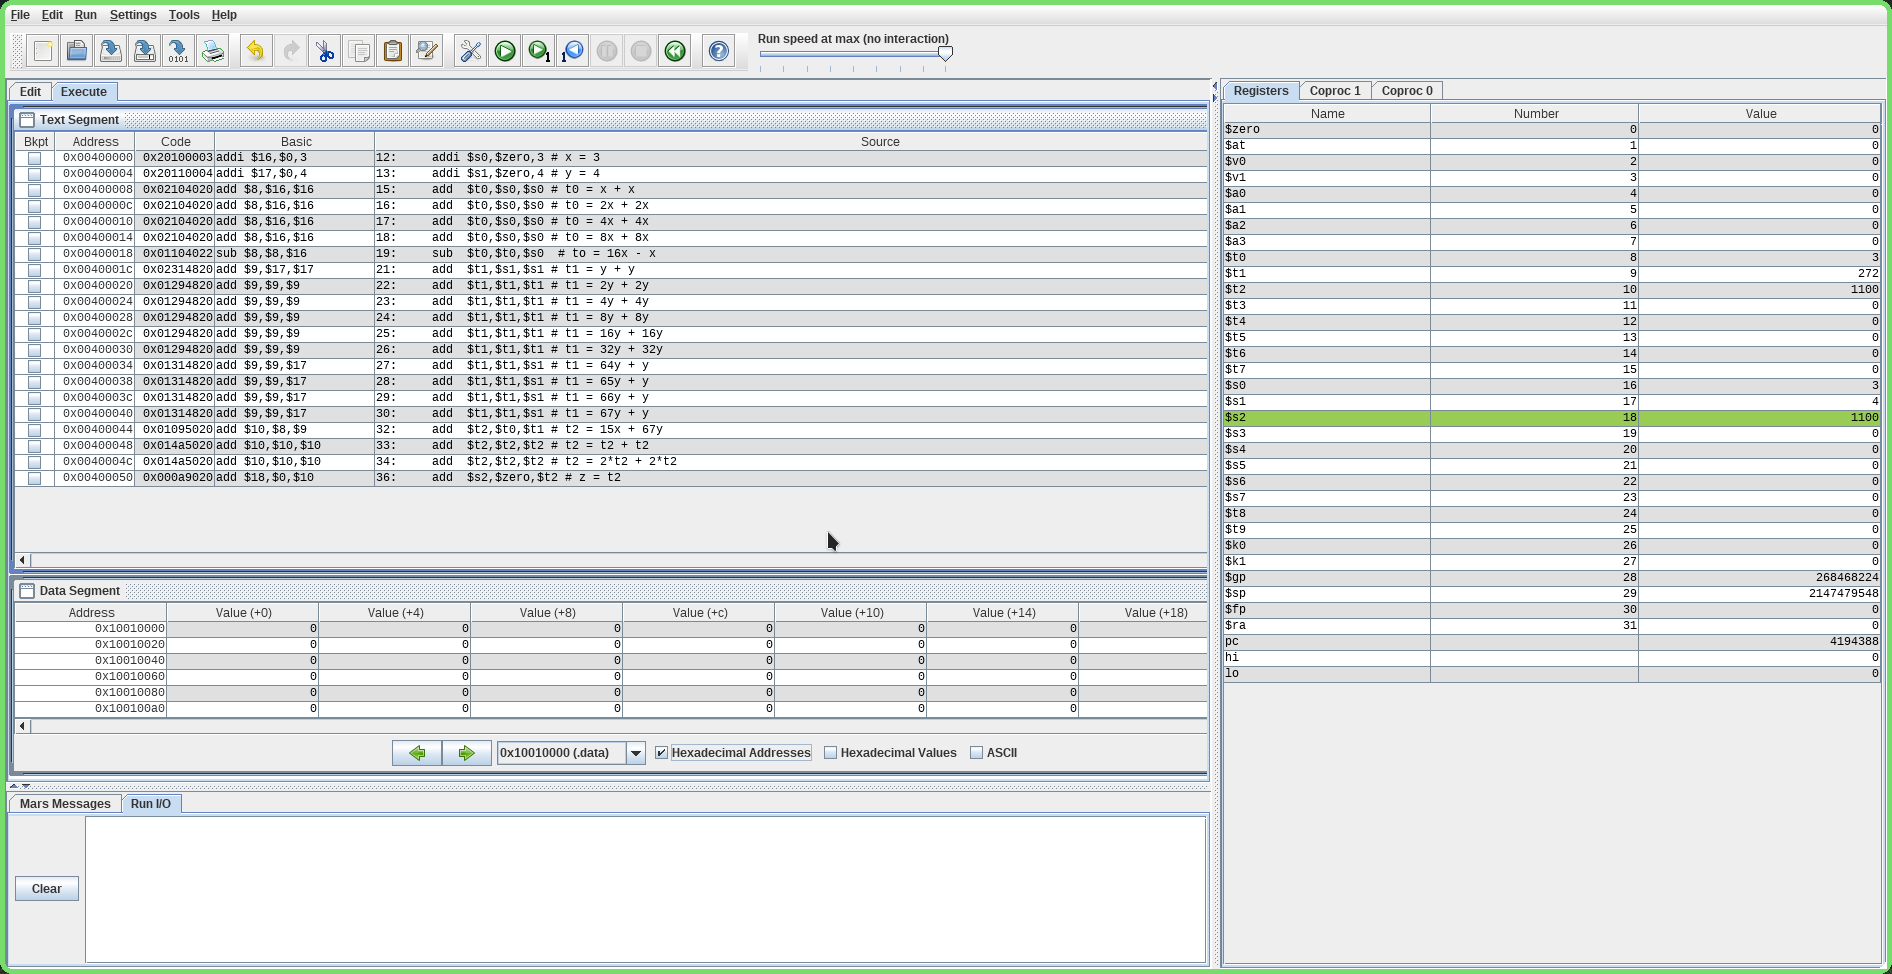
\includegraphics[width=1\textwidth]{programa3}
\end{figure} 
\begin{figure}[!ht]
    \caption{Programa 4}
    \centering
    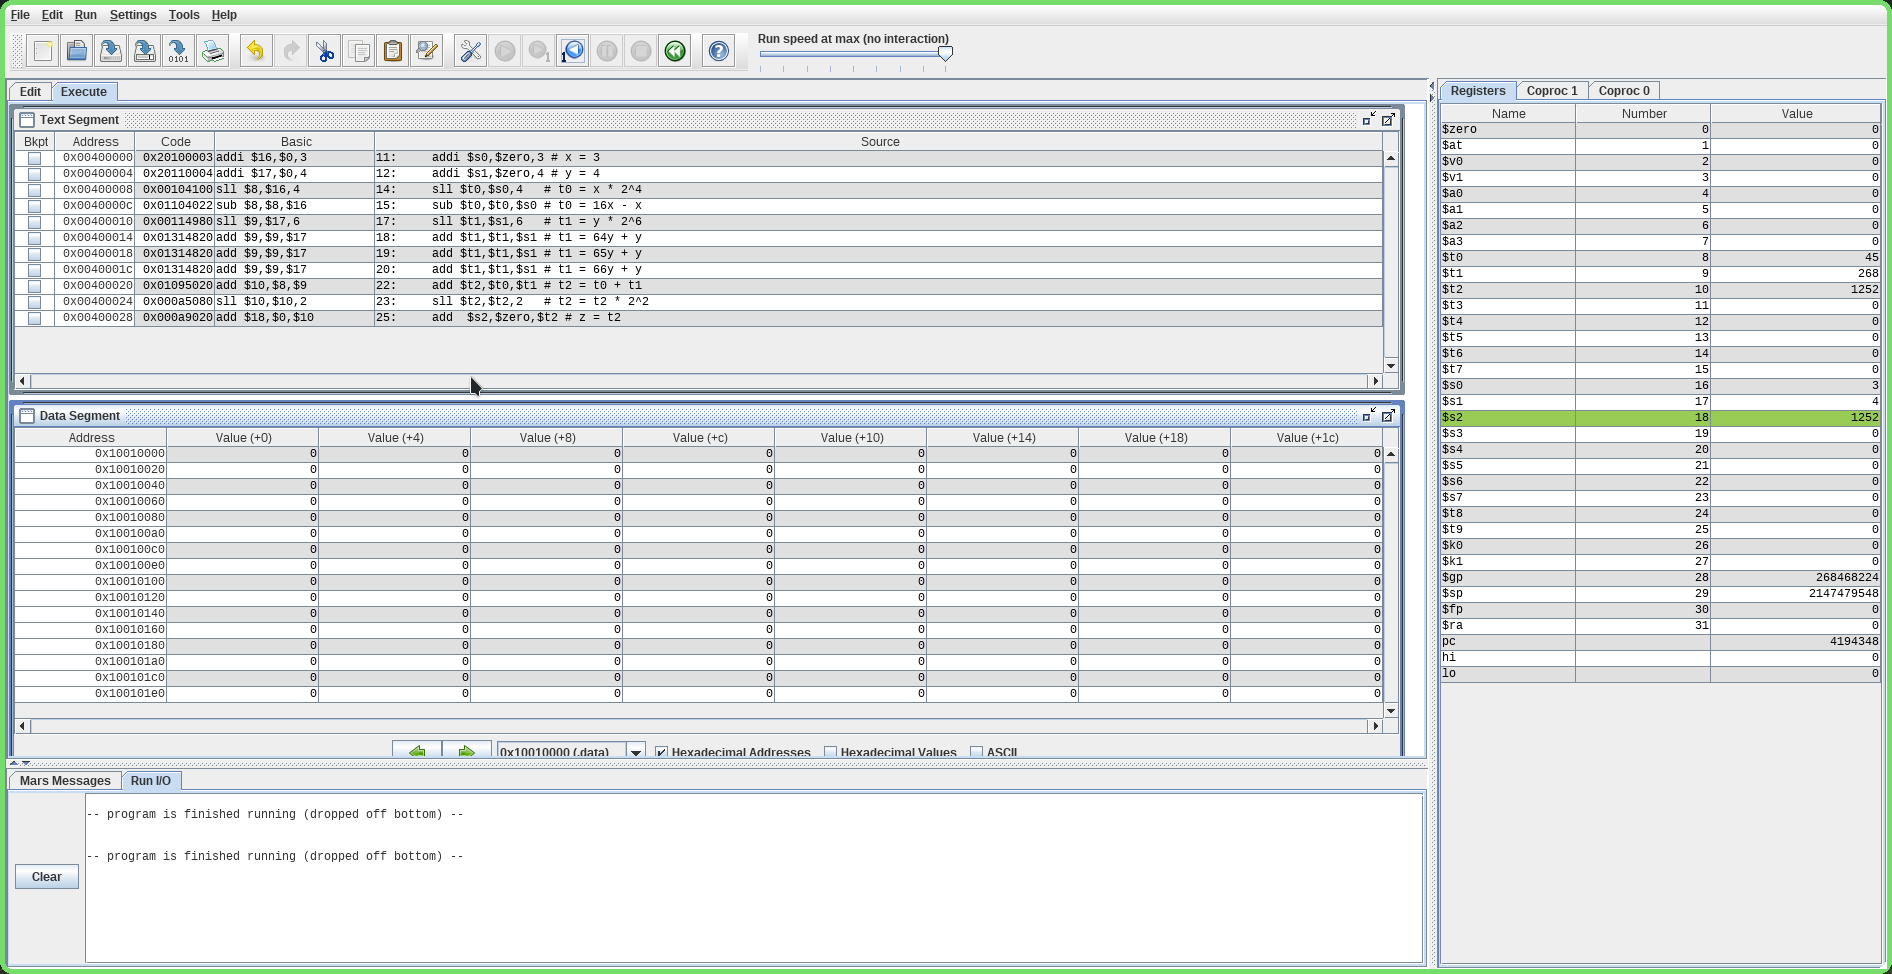
\includegraphics[width=1\textwidth]{programa4}
\end{figure} 
\begin{figure}[!ht]
    \caption{Programa 5}
    \centering
    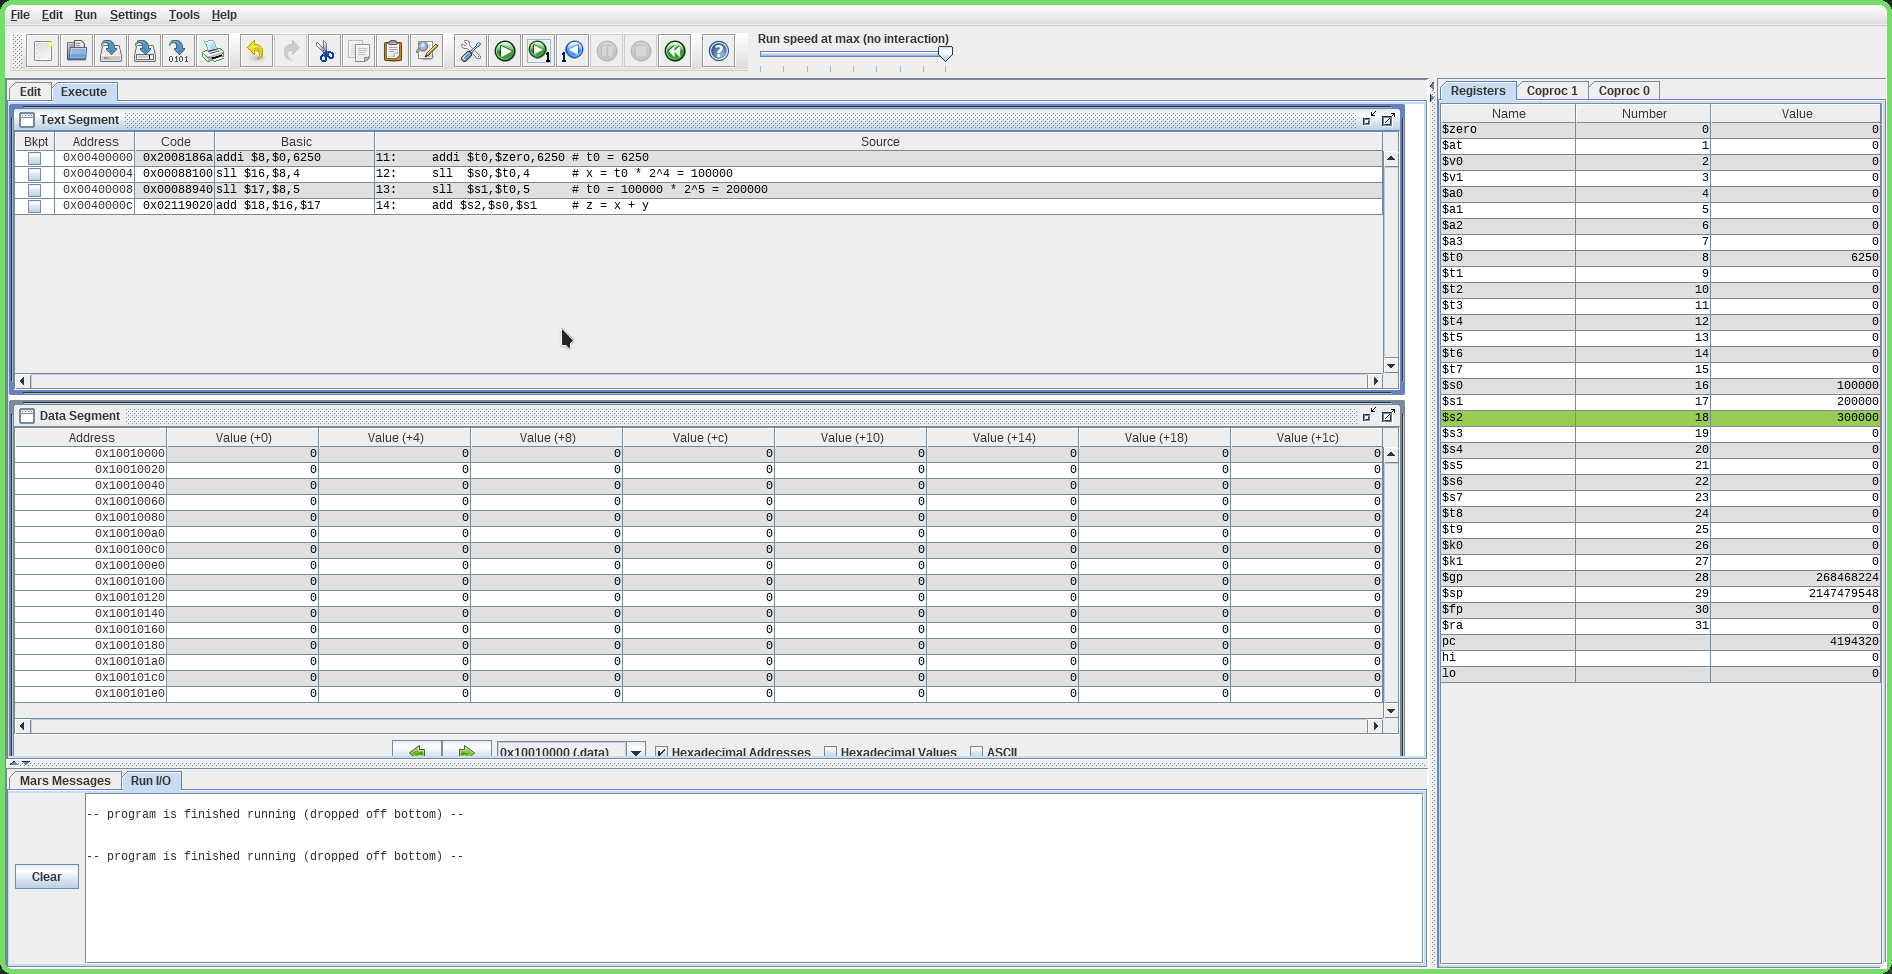
\includegraphics[width=1\textwidth]{programa5}
\end{figure} 
\begin{figure}[!ht]
    \caption{Programa 6}
    \centering
    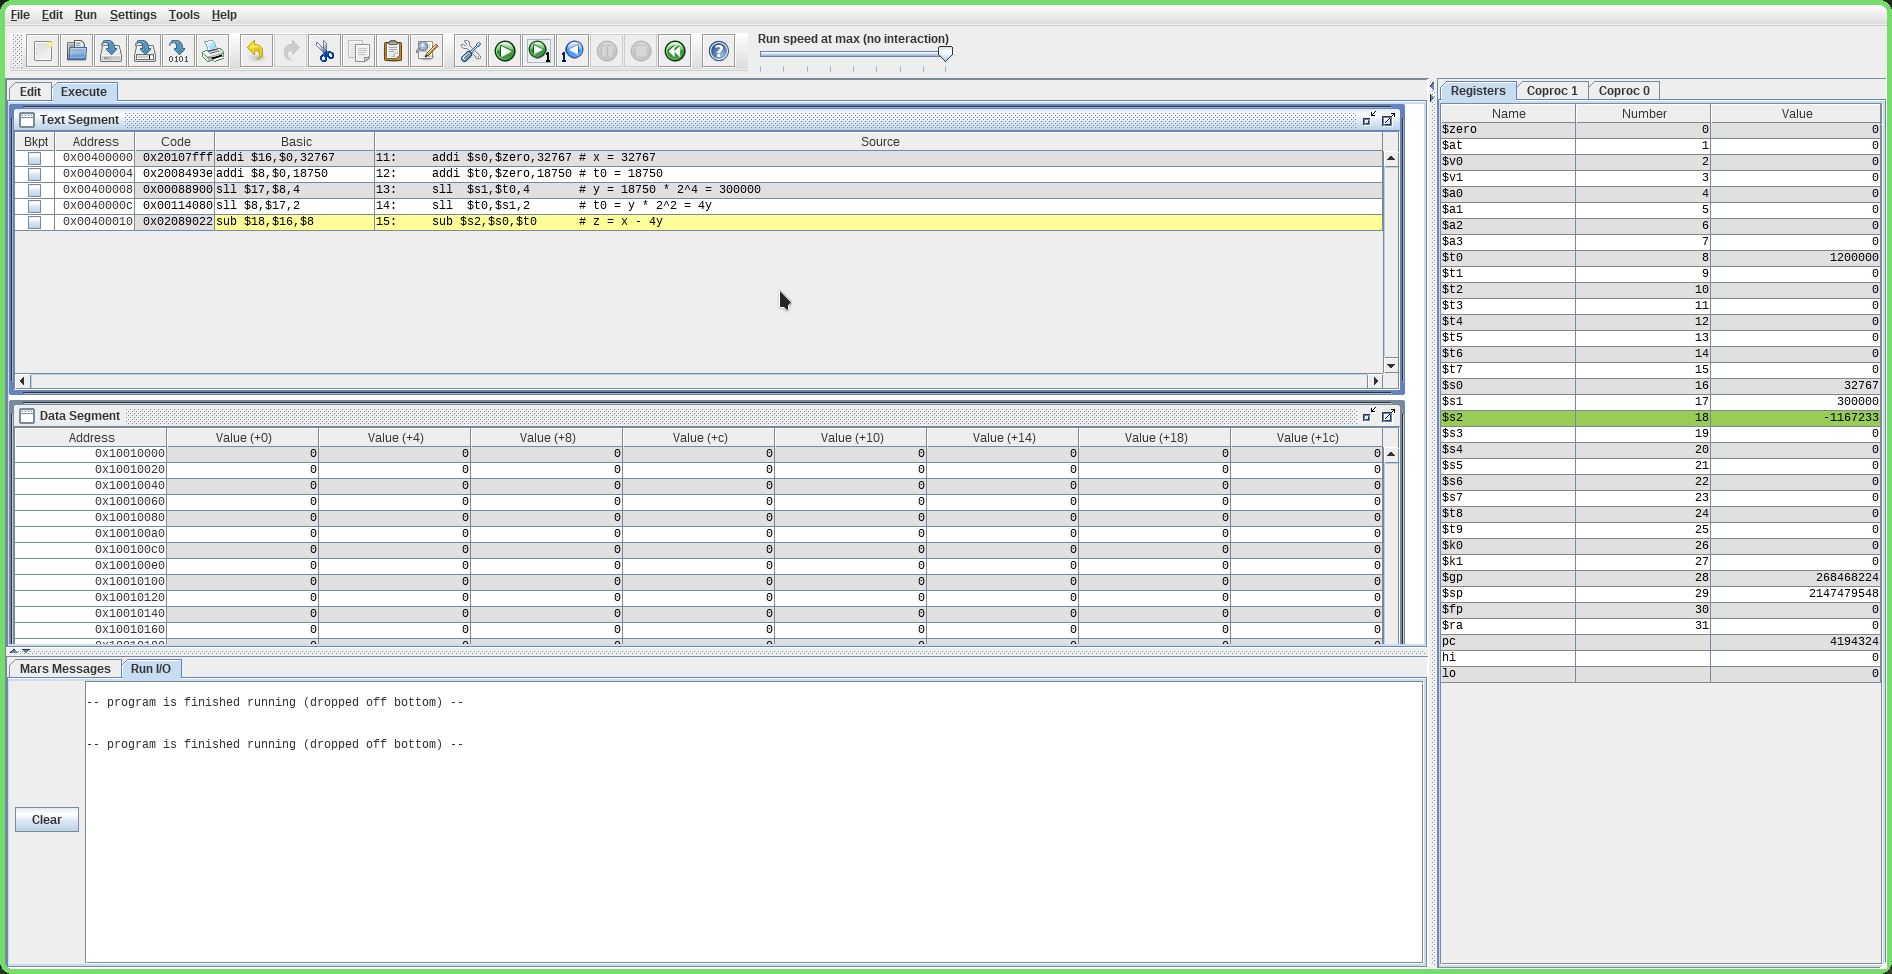
\includegraphics[width=1\textwidth]{programa6}
\end{figure} 
\begin{figure}[!ht]
    \caption{Programa 7}
    \centering
    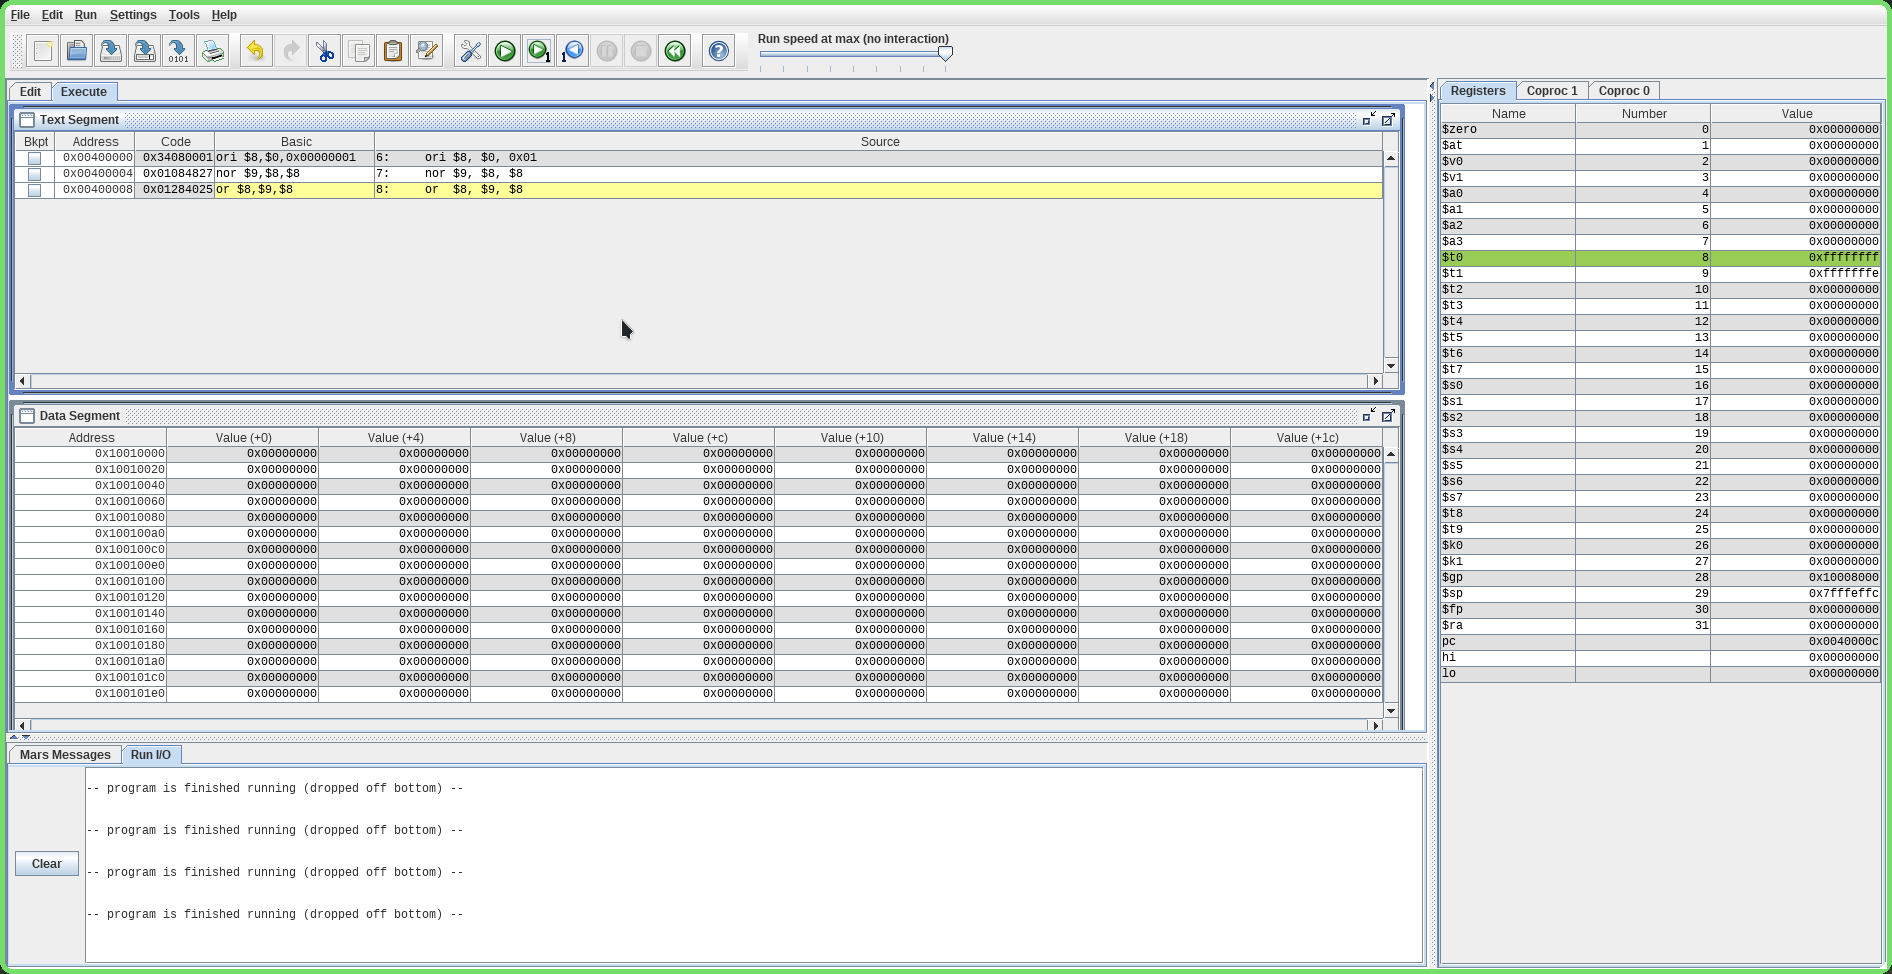
\includegraphics[width=1\textwidth]{programa7}
\end{figure} 
\begin{figure}[!ht]
    \caption{Programa 8}
    \centering
    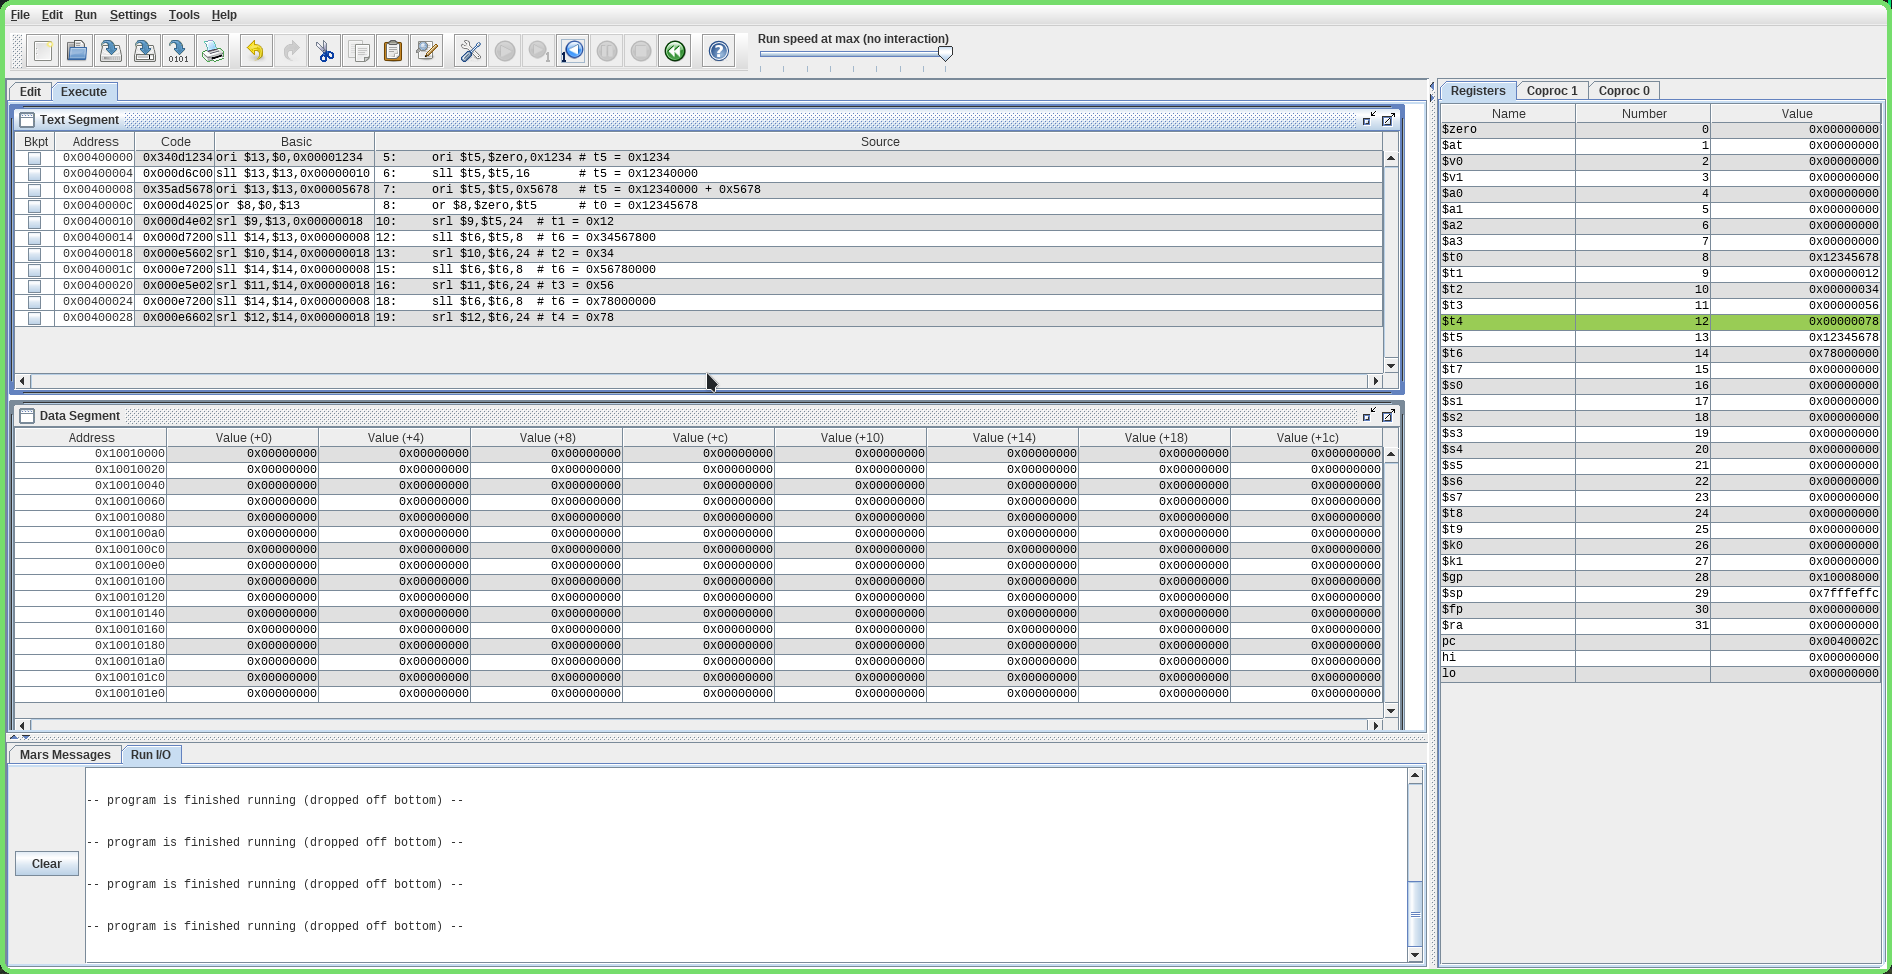
\includegraphics[width=1\textwidth]{programa8}
\end{figure}  
\end{document}
